This chapter details the implementation of the automated solution proposed in Chapter \ref{chap:context}. First, an overview of the various components implemented throughout the project is given. Next, the implementation of a deep network capable of automatically extracting annual density bands present in two dimensional data is discussed. The attempts at implementing a network capable of automatically extracting the annual density bands present in three dimensions are also detailed. Then, the implementation of and reasoning behind the custom accuracy metric is discussed. Finally, the techniques used to estimate the calcification rate from the extracted boundaries are described.

\section{Overview}

A system capable of calculating the calcification rate given only some section of density data requires the implementation of many separate subcomponents. Figure \ref{fig:overview} provides an overview of these components and outlines the order in which they were implemented and will be discussed. Ultimately, the training of a 2D architecture to predict the positions of the boundaries between annual density bands was the main focus of the project. The steps taken to implement this component compose the majority of the content in this Chapter.

All aspects of the project relied heavily on the provided dataset. The processing and labelling of the data was a significant part of the implementation and will be discussed in detail. An example of a 3D scan present in the dataset is shown in Figure \ref{fig:scanexample}.

\begin{figure}[!b]
    \centering
    \begin{subfigure}[t]{0.49\textwidth}
        \centering
        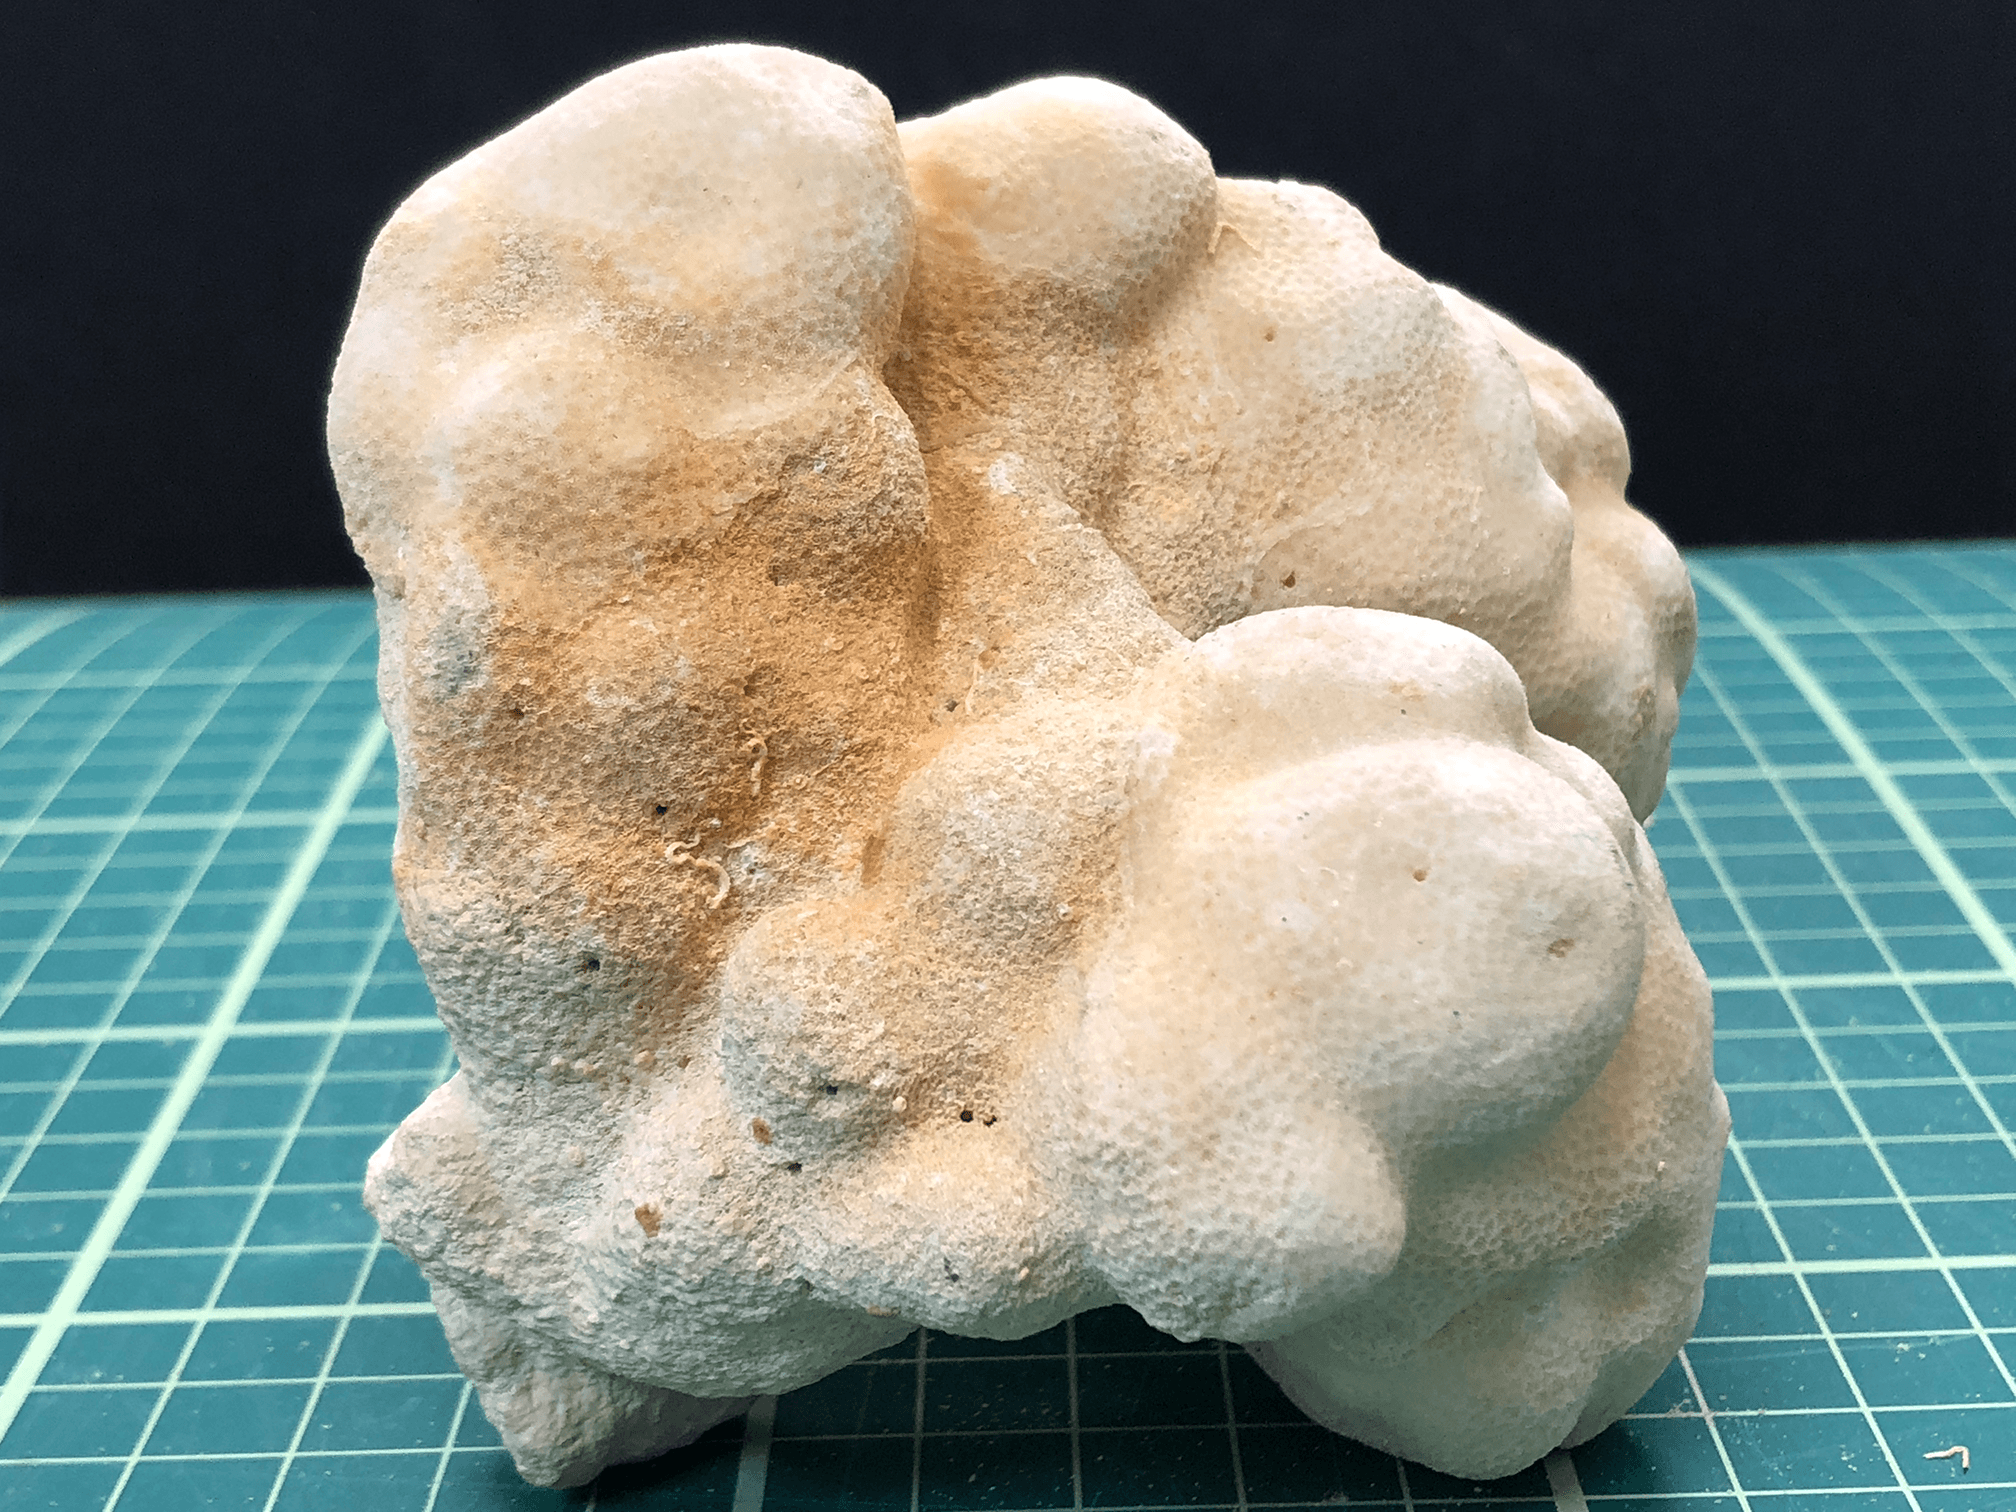
\includegraphics[width=1\textwidth, valign=c]{images/real-coral.png}
    \end{subfigure}
    ~
    \begin{subfigure}[t]{0.49\textwidth}
        \centering
        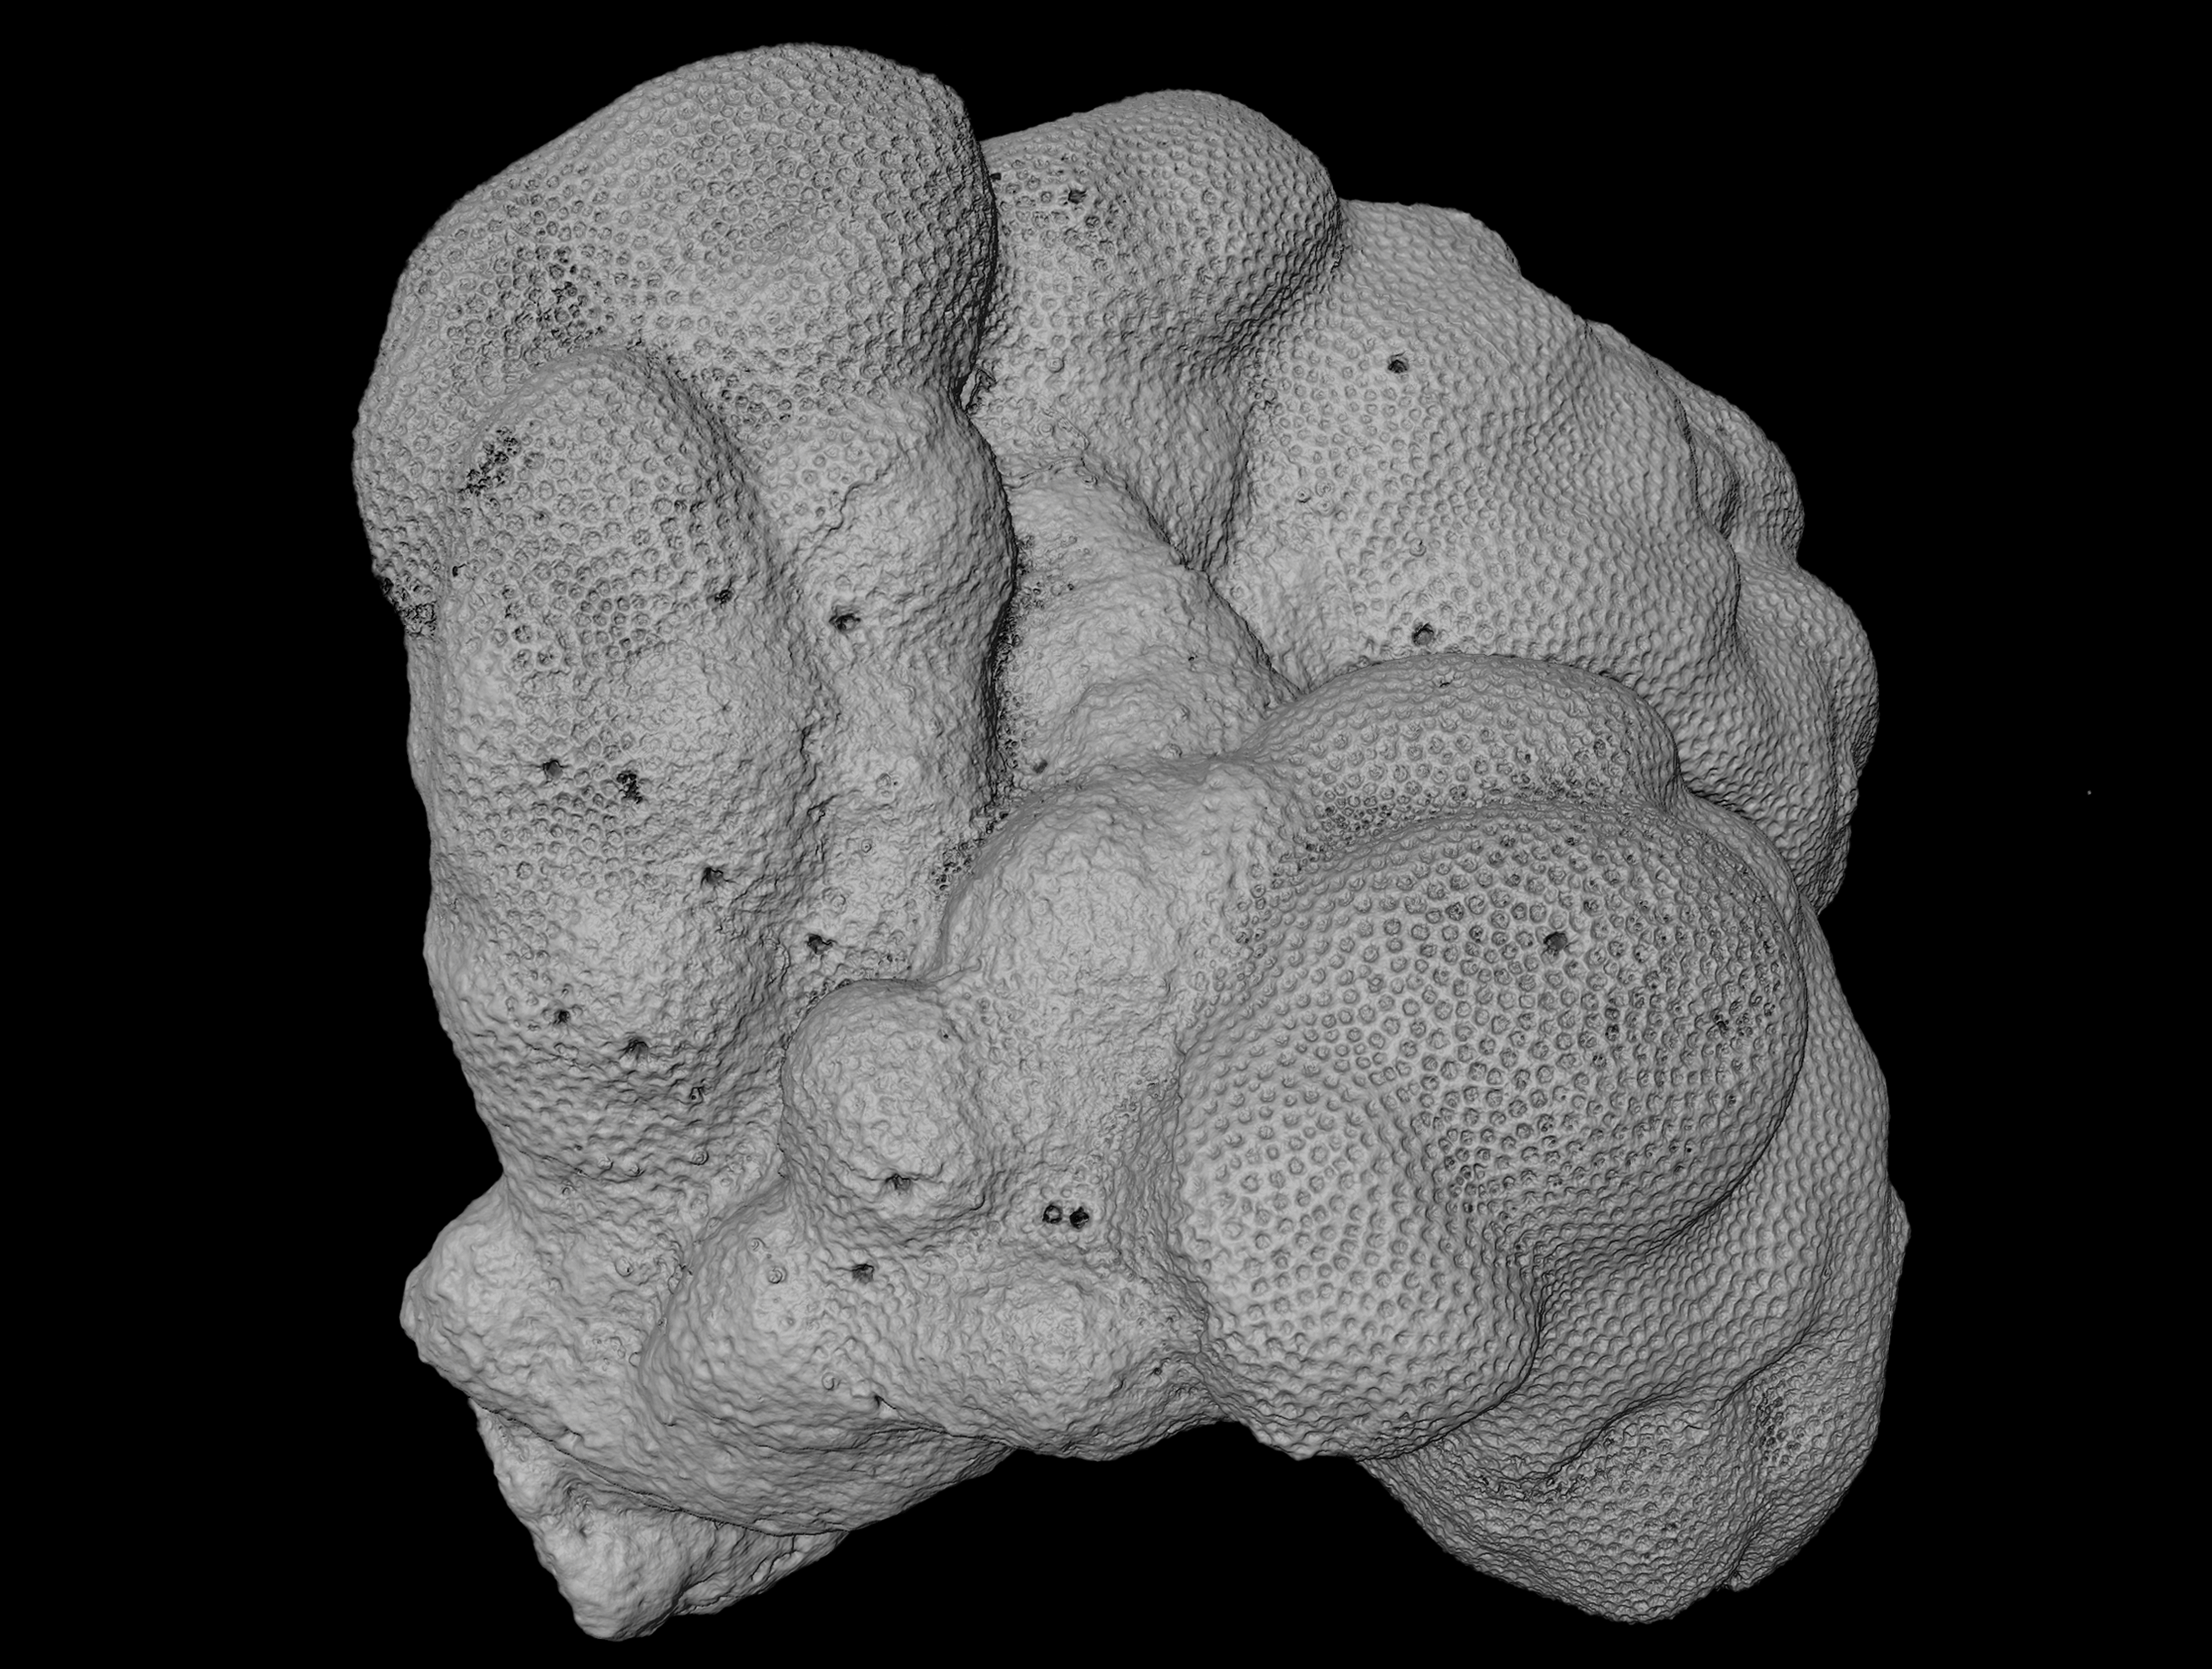
\includegraphics[width=1\textwidth, valign=c]{images/3D-scan.png}
    \end{subfigure}
    \caption{\textbf{(left)} An example of a Porites coral skeleton from the Natural History Museum's collection. This particular sample was collected from the Solomon Islands in 1974. In the initial dataset, the scan of this sample is represented by 1945$\times$1508$\times$1208 voxels. \textbf{(right)} A 3D volume rendering of the CT scan of the sample shown on the left. Created using the Avizo software package.}
    \label{fig:scanexample}
\end{figure}

\begin{figure}[!p]
    \centering
    \includegraphics[width=\textwidth, height=1.45\textwidth]{example-image-a}
    \caption{A diagram providing an overview of the components implemented throughout the project.}
    \label{fig:overview}
\end{figure}

\begin{figure}[!t]
    \centering
    \begin{subfigure}[t]{0.49\textwidth}
        \centering
        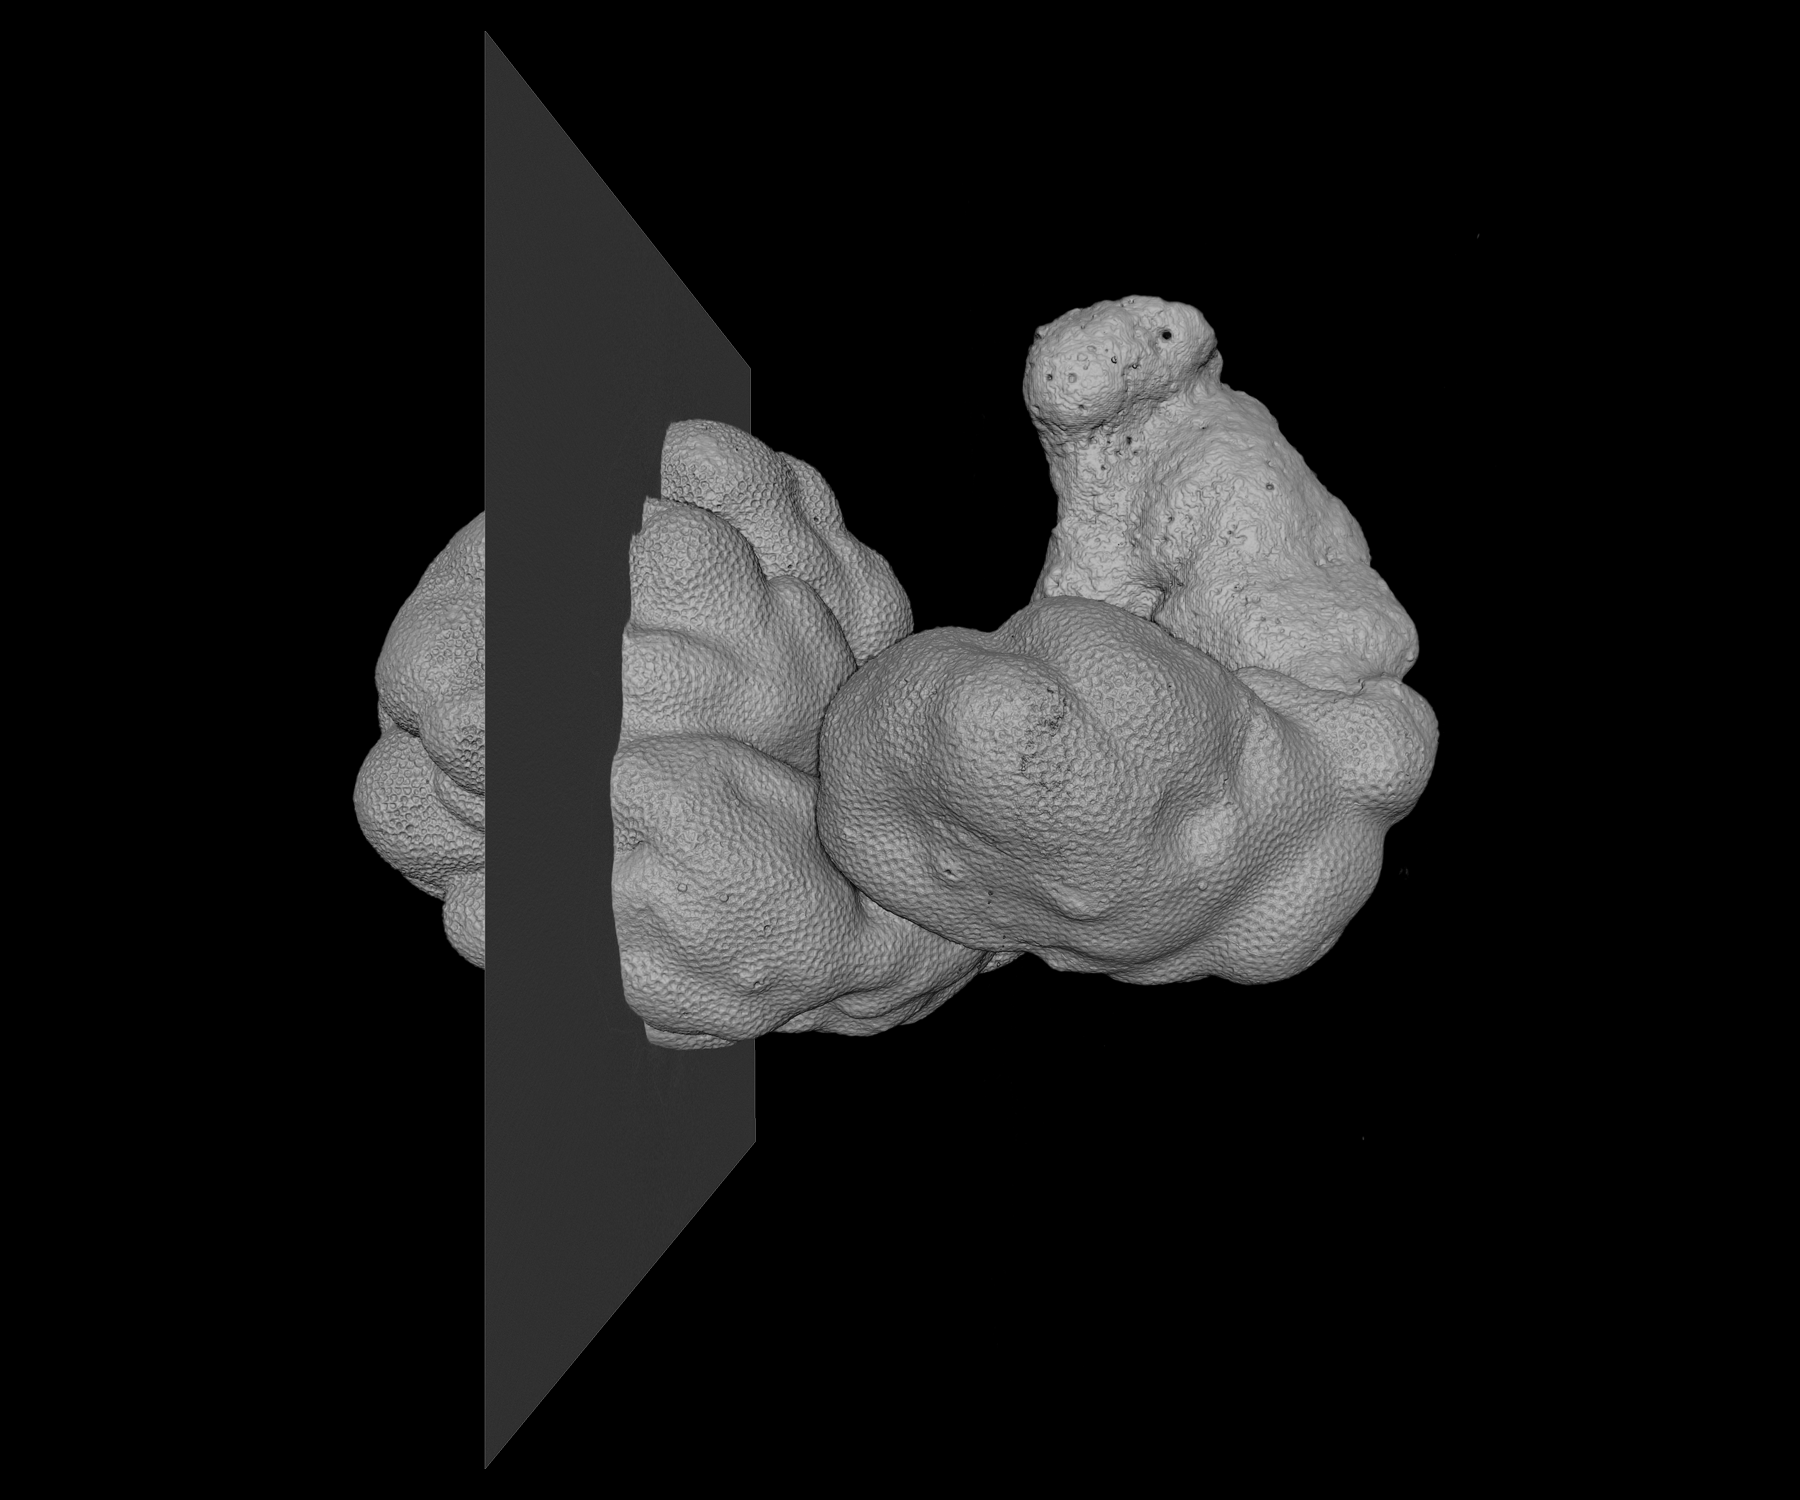
\includegraphics[width=1\textwidth, valign=c]{images/extraction.png}
    \end{subfigure}
    ~
    \begin{subfigure}[t]{0.49\textwidth}
        \centering
        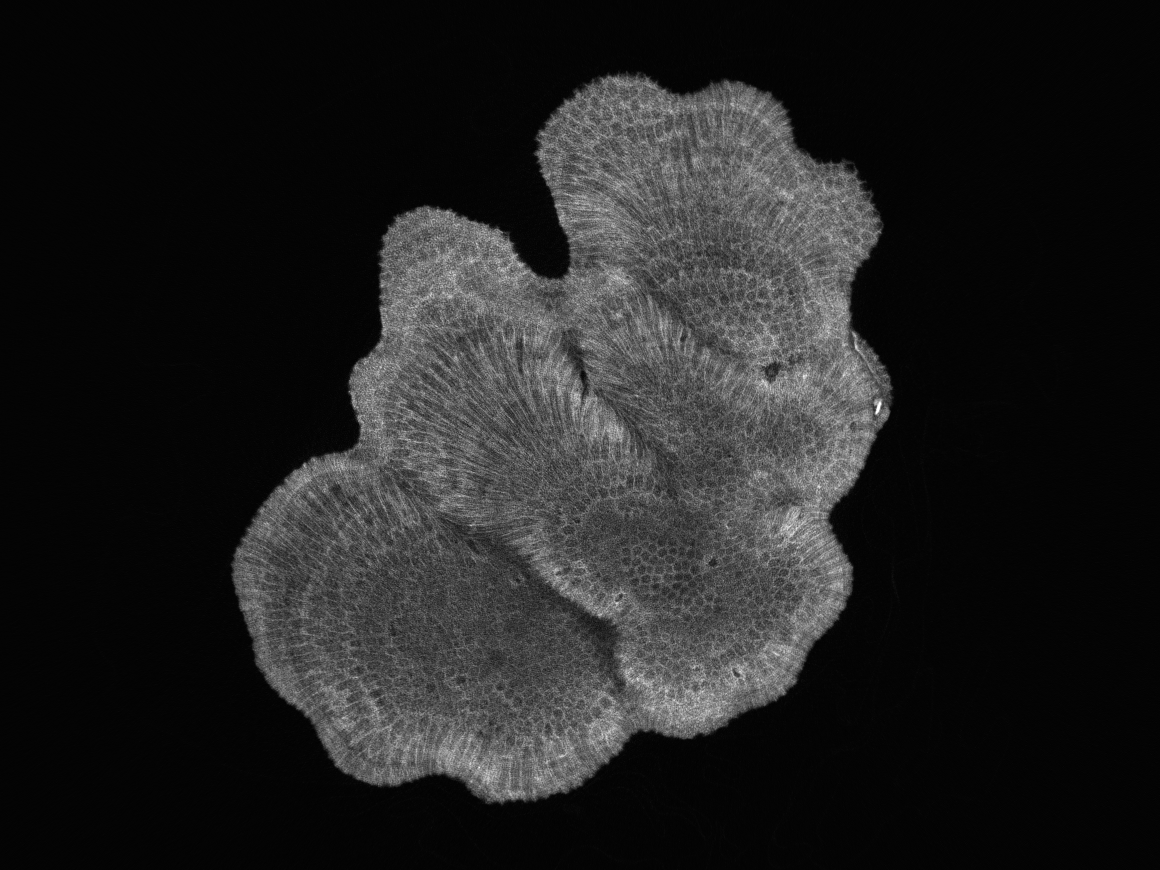
\includegraphics[width=1\textwidth, valign=c]{images/slice-example.png}
    \end{subfigure}
    \caption{An illustration of the how the 3D CT data is composed of many 2D slices. \textbf{(left)} A 3D volume rendering of one of the CT scans present in the dataset. The grey rectangle ``cuts'' the scan and produces the slice shown on the right. It can also be seen that the scan on the left is represented by many slices similar to the one shown on the right. \textbf{(right)} A 2D slice extracted from the CT scan shown on the left. The slice is a negative; brighter pixels correspond to high density and darker pixels correspond to low density.}
    \label{fig:extraction}
\end{figure}

\section{Two Dimensional Boundary Extraction}

This section outlines the steps taken to implement and train a CNN capable of extracting the annual density banding present in two dimensional data.

\subsection{Labelling the Data}
\label{sec:2dlabel}

In order for a supervised CNN to perform well, large amounts of labelled data must be available to train on. Since the dataset provided was initially unlabelled, a manual labelling process was devised and is described in this section.

\subsubsection{The Initial Dataset}

The dataset provided contains more than 160 three dimensional computed tomography (CT) scans of unique coral skeletons from the Natural History Museum's collection. Each individual 3D scan consists of stacks of thousands of 2D \texttt{.tif} images which will be referred to as ``slices'' (see Figure \ref{fig:extraction}). This unlabelled dataset will be referred to as the ``initial dataset''. Although the initial dataset contains scans of ten different genera of coral, only scans of the Porites genus were considered for labelling and training the network with. An example of a Porites skeleton that is part of the dataset is shown in Figure \ref{fig:scanexample}. The Porites scans were chosen as they contain annual banding that can be more easily identified and labelled when compared to other coral genera.

A typical scan consists of ${\sim}2000$ slices that each have the same resolution of ${\sim}$2000$\times$2000 pixels resulting in an overall 3D resolution of 2000$\times$2000$\times$2000 voxels. The 3D resolution of each scan varies, but the scale (e.g., the number of voxels used to represent a centimetre cubed) is consistent across scans.

\begin{figure}[t]
    \centering
    \begin{subfigure}[t]{0.49\textwidth}
        \centering
        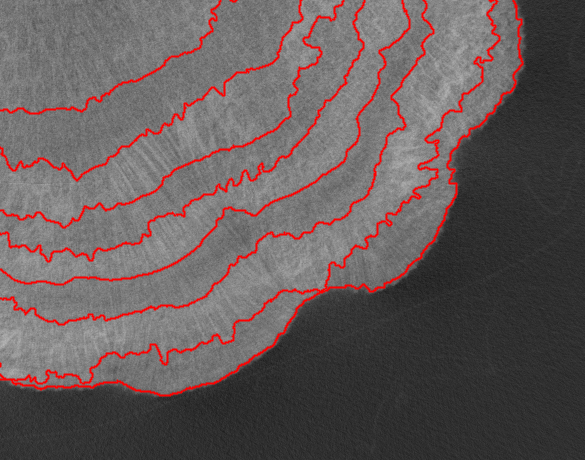
\includegraphics[width=1\textwidth, valign=c]{images/rough-label.png}
    \end{subfigure}
    ~
    \begin{subfigure}[t]{0.49\textwidth}
        \centering
        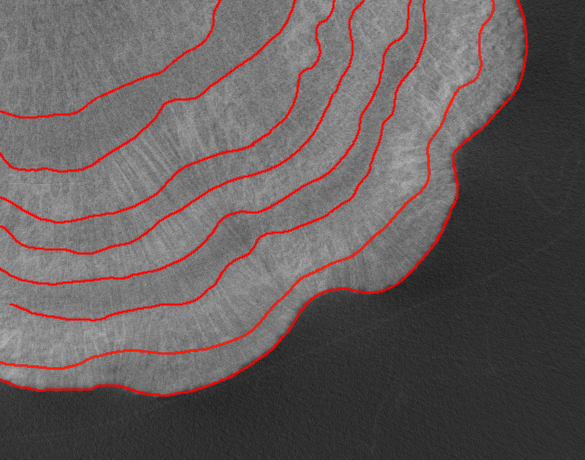
\includegraphics[width=1\textwidth, valign=c]{images/smooth-label.png}
    \end{subfigure}
    \caption{A comparison of the two methods of labelling that were initially considered. The boundary labels are coloured red and placed over the the same original negative 2D slice. \textbf{(left)} A method of labelling in which the boundaries were placed at the sharpest change in density resulting in complex boundaries whose positions are highly sensitive to noise in the image. \textbf{(right)} A method in which the chosen boundaries are ``smooth'' whilst also being placed as close as possible to the sharpest changes in density.}
    \label{fig:labelstyle}
\end{figure}

\subsubsection{Slice Selection and Extraction}

Not all slices that compose a scan contain annual density banding that can confidently be identified. In order to find appropriate slices, each Porites scan was opened and inspected manually using a 3D visualisation program called Avizo\footnote{\url{https://tiny.cc/avizo}}. Avizo allows users to view slices orthogonal to the $x$, $y$, or $z$ axis of a scan. A selection of six slices that could confidently be labelled were chosen. Since the density banding boundaries are orthogonal to the growth direction (or ``concordant'' with the growth surface~\cite{knutson}), the slices that present the most obvious density banding are normally parallel to the direction of growth. Once these slices were identified, a Python script was used to extract each slice and export them as greyscale \texttt{.png} images. The slices can be represented as greyscale images since they only require one channel to represent depth. Some of the surrounding slices were also extracted in order to curate the 3D dataset used later in the project (discussed in Section~\ref{sec:threedimension}).

\subsubsection{Slice Labelling}

Once the slices were selected, a labelling process was established. Initially, two methods of labelling were considered and shown to Dr Erica Hendy, a senior lecturer in biogeochemical cycles. Of the two methods (shown in Figure \ref{fig:labelstyle}), the ``smooth'' method was deemed as the more realistic choice. An idealised annual density cycle is actually in the form of a sinusoidal wave with the density gradually changing from high to low and back over the course of a year~\cite[p. 39]{coralsine}. Thus, an exact boundary between a high and low band does not actually exist, making the ``complex'' method unrealistic both in terms of reproducibility, and in terms of biological accuracy.

Each selected slice was then manually labelled using the GNU Image Manipulation Program (GIMP)\footnote{\url{https://www.gimp.org}}. A one pixel wide white line is drawn at the beginning and end of each annual high density band and the rest of the image is black---no values other than black or white are present in the labels. In order to ensure that the decisions made regarding the boundaries of the annual bands were as consistent as possible, each slice was manually labelled three or more times, and the most common boundaries were chosen. It is important for the labelling method to be consistent and reproducible as this enables the dataset to be more easily expanded in the future.

\subsection{Dataset Curation}
\label{sec:datasetcuration}

With only a small selection of slices successfully extracted and labelled, a larger dataset of image-label pairs was required for the model to train on.

\subsubsection{Sliding Window}

In order to expand the dataset, a sliding window technique was used. A script was written in Python that took a slice, two 2D coordinates, a ``stride'', and a size as arguments. The pair of coordinates corresponded to the top left corner and bottom right corner of the confidently labelled area of the slice. This was the area that the window would slide over in order to create the resulting ``patches''. The stride argument dictated how far the window should slide before each patch was produced. The most common stride value used was 20. The size argument defined how large the resulting patches should be. The patches initially produced had a resolution of 256$\times$256 pixels, but various sizes of patches were experimented with and are discussed in Chapter \ref{chap:evaluation}. The arguments used in order to produce the curated dataset used in this project are shown in Table \ref{tab:slidingwindow}. A total of 388 patches were produced from six slices taken from four different coral skeleton scans. This dataset of 388 256$\times$256 patches and their corresponding labels were stored as greyscale \texttt{.png} images.

\begin{table}[t]
\centering
\caption{A table showing the arguments used with the Python script for each labelled slice. For each slice, a size argument of 256 was also specified. Note that some slices are represented by two rows as these slices contained two separate areas that could be confidently labelled. It was not possible to use one area that contains the two areas as this would result in multiple patches with no labelling being produced.}
\begin{tabular}{@{}lrrrrrr@{}}
\toprule
Slice & $x_{top}$ & $y_{top}$ & $x_{bottom}$ & $y_{bottom}$ & Stride (px) & Patches produced \\ \midrule
RS0030\_yz\_0625.tif    & 1028      & 153       & 1350         & 530          & 20          & 36      \\
RS0030\_yz\_0642.tif    & 1070      & 143       & 1390         & 463          & 20          & 18      \\
RS0030\_yz\_0642.tif    & 895       & 400       & 1275         & 685          & 20          & 12      \\
RS0116\_0414.tif        & 666       & 1258      & 1560         & 1750         & 40          & 150     \\
RS0116\_0500.tif        & 970       & 1320      & 1320         & 1854         & 30          & 54      \\
RS0116\_0500.tif        & 1130      & 1250      & 1525         & 1730         & 30          & 56      \\
RS0128\_yz\_0451.tif    & 490       & 258       & 790          & 690          & 20          & 32      \\
RS0130\_xz\_0820.tif    & 513       & 1190      & 828          & 1485         & 10          & 30      \\ \midrule
Total                   &           &           &              &              &             & 388     \\ \bottomrule
\end{tabular}
\label{tab:slidingwindow}
\end{table}

In order to prevent the dataset from representing certain coral samples better than others, an effort was made to equalise the number of patches produced per scan. Due to different slices containing varying sizes of confidently labelled areas, the stride argument was used to increase or reduce the number of patches produced. However, it was also important to produce as much data as possible to enable the network to perform well. Ultimately, some slices produced almost five times as many slices as others resulting in some imbalance in the types of coral scans represented by the dataset. Although this could negatively affect the generalisability of a network trained on this dataset, cross-validation with carefully selected splits to represent each coral scan was ultimately used and is discussed in Chapter \ref{chap:evaluation}.

\subsubsection{Splitting the Dataset}

For the initial training and testing of the network, the curated dataset was split into a training set, a validation set, and a test set. Of the 388 patches, 322 were used for training, 56 for testing, and 10 for validation. The patches composing the test and validation sets were all produced from slices of a coral skeleton that was not part of the training set. This ensured that the network could not have been overfitting to the nature of the annual banding present in the skeleton used for testing. If this had been the case, the performance on the test data could have been positively skewed.

\subsection{Data Augmentation}

As discussed in Chapter \ref{chap:technical}, data augmentation is an important regularization technique. Since only 388 patches had been produced, extensive augmentation was used to artificially expand the dataset. This data augmentation later proved effective in improving the performance achieved by the network and is discussed further in Chapter \ref{chap:evaluation}.

\subsubsection{The Keras \texttt{ImageDataGenerator} class}

The Keras library allows users to easily implement augmentation using the \texttt{ImageDataGenerator} class\footnote{\url{https://keras.io/preprocessing/image}}. In this case, the \texttt{flow\_from\_directory} method was used to perform online augmentation. This method first loads images from a directory into batches. A series of random transformations are then applied to each batch. These original batches are then replaced with the new randomly transformed versions. The \texttt{flow\_from\_directory} method then returns a Python generator that will yield randomly augmented batches of the data indefinitely. A network trained on the generator produced by this method will therefore be trained on randomly transformed samples as opposed to the original samples themselves. The batches can then be input to the model in the form of $(batch \times y \times x \times 1)$ tensors where $batch$ is the batch size, $y$ and $x$ are the heights and widths of the patches respectively, and 1 is the number of channels (since the patches are stored as greyscale images).

The \texttt{flow\_from\_directory} method only loads one stream of images from a directory. In order to load the corresponding labels from another directory, a \texttt{flow\_from\_directory} method from another instance of the \texttt{ImageDataGenerator} class must be used. The two generators produced can then be ``zipped'' into a single generator that yields image-label pairs.

Since the \texttt{flow\_from\_directory} method applies random transformations to each image, the same random transformations must also be applied to the corresponding labels. This can be achieved by passing the same \texttt{seed} argument to the two \texttt{flow\_from\_directory} methods used to load the images and labels. These methods are also capable of shuffling the order in which images are loaded and trained with, so using the same \texttt{seed} value also ensures that the shuffling follows the same order for both the images and labels. The actual transformations to be used when augmenting the data are specified using various arguments passed to the \texttt{ImageDataGenerator} constructor.

Since the training generator will yield randomly augmented image-label pairs indefinitely, a ``classic'' epoch will never be completed. Instead, when training the network the \texttt{steps\-per-epoch} argument defines how many samples should be processed before an epoch is considered complete. A simplified example demonstrating the implementation of the training generator and the transformations used is shown in Listing \ref{lst:augment}.

\subsubsection{Acceptable Augmentations}

The possible transformations specified each have a random chance of being applied to each image. It was important to choose a range of possible transformations that would always produce a reasonable augmented image. The permitted augmentations that could be randomly chosen were:

\begin{itemize}
    \item Rotations within a range of $\pm 2$ degrees.
    \item Shifts in the $x$ axis within a range of $\pm 2\%$ of the images' widths.
    \item Shifts in the $y$ axis within a range of $\pm 2\%$ of the images' heights.
    \item Shears within a range of $\pm 2$ degrees.
    \item Zooms in the $x$ and $y$ axes within a range of $\pm 2\%$ of the images' widths or heights.
    \item Brightness shifts within a range of $\pm 10\%$.
    \item Horizontal flips.
    \item Vertical flips.
\end{itemize}

Using larger ranges of permitted transformations resulted in augmented images that did not represent the real data well. Examples of images created using both the ranges defined above and ``unrealistic'' ranges are shown in Figure \ref{fig:augexample}.

\begin{figure}[t]
    \centering
    \begin{subfigure}[t]{0.18\textwidth}
        \centering
        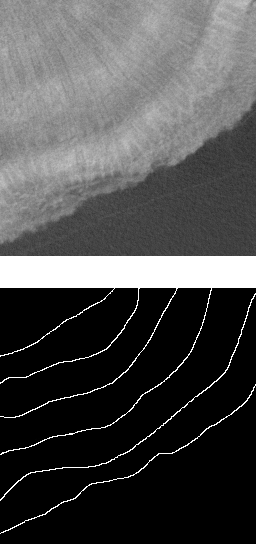
\includegraphics[width=1\textwidth, valign=c]{images/orig-aug.png}
        \caption{Original}
    \end{subfigure}
    ~
    \begin{subfigure}[t]{0.38\textwidth}
        \centering
        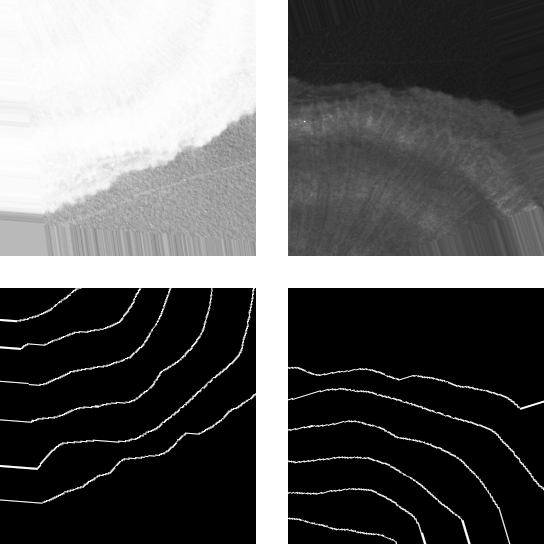
\includegraphics[width=1\textwidth, valign=c]{images/bad-aug.png}
        \caption{Unrealistic}
    \end{subfigure}
    ~
    \begin{subfigure}[t]{0.38\textwidth}
        \centering
        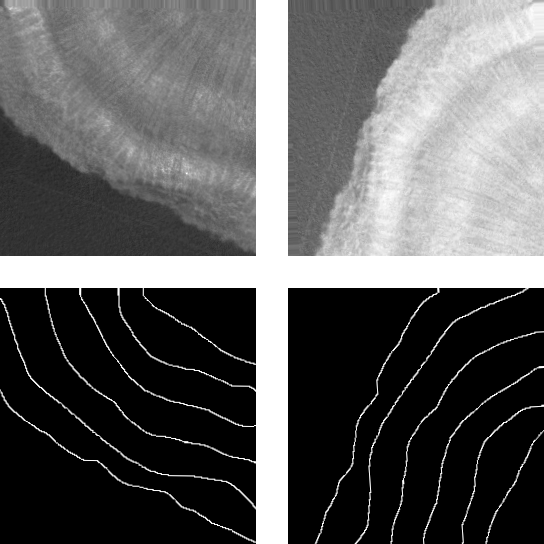
\includegraphics[width=1\textwidth, valign=c]{images/good-aug.png}
        \caption{Realistic}
    \end{subfigure}
    \caption{Examples of augmented images created using both ``unrealistic'' and ``realistic'' sets of permitted transformations. The images are shown at the top and their corresponding labels are shown at the bottom. All labels are thresholded after augmentation to ensure that only white or black values are present. \textbf{(a)} The original image-label pair. \textbf{(b)} Two examples of image-label pairs augmented using a set of unrealistic permitted transformations resulting in images that do not represent the real coral data well. The first image's brightness has been shifted too far and the overly aggressive rotation and shifting has resulted in straight labels on the left-most edge which are not realistic. The second image's label has also been rotated too far resulting in a straight label on the right-most edge. \textbf{(c)} Two examples of image-label pairs augmented using the set of permitted transformations used in this project.}
    \label{fig:augexample}
\end{figure}

\subsection{U-Net}

As discussed in Chapter \ref{chap:technical}, the U-Net architecture~\cite{ronneberger2015u} is the main architecture experimented with. The implementation used throughout the project was initially based off of an implementation available on GitHub\footnote{\url{https://github.com/zhixuhao/unet}}, though over the course of the project the majority of the code has been edited. It is written in Python and makes use of the Keras functional API. Recall that the original U-Net architecture consists of three sections: the contracting path, the bottleneck, and the expanding path. A high level diagram of the U-Net architecture is shown in Figure \ref{fig:unetushape} and can be used to better understand the implementation details described.

\subsubsection{The Contracting Path}

The contracting path consists of multiple ``blocks'' with each block consisting of two convolutional layers followed by a 2$\times$2 max-pooling layer with a stride of two. The convolutional layers both use 3$\times$3 kernels and the ReLU activation function. Apart from the first block, the first convolutional layer of each contracting block doubles the number of feature channels. The implementation of the first contracting block is shown in Listing \ref{lst:block1}.

\begin{lstlisting}[float={!t},caption={IThe implementation of the first contracting block of the U-Net architecture using the Keras functional API.},label={lst:block1},language=Python,upquote=true,belowskip=0pt]
conv1 = Conv2D(64, 3, activation="relu", padding="same")(inputs)
conv1 = Conv2D(64, 3, activation="relu", padding="same")(conv1)
pool1 = MaxPooling2D(pool_size=(2, 2))(conv1)
\end{lstlisting}
The \texttt{pool1} tensor defined in Listing \ref{lst:block1} will be the input to the next contracting block, and so on. The first argument of the \texttt{Conv2D} function is the number of output feature channels. Since the number of feature channels doubles at each contracting block, the next contracting block would have two convolutional layers outputting 128 feature channels rather than 64. The second argument is the size of convolutional kernels to use, so 3$\times$3 in this case. Note that the Keras \texttt{MaxPooling2D} function implicitly uses the same stride size as the pool size specified, so a stride of two in the $x$ and $y$ axes will be used.

The \texttt{"{}same"{}} padding argument specifies that the dimensions of the output feature channels should match the dimensions of the inputs. This differs from the implementation of the U-Net architecture used in the original paper. The original U-Net architecture would start with an oversized input. For example, to segment a 388$\times$388 image, a 572$\times$572 image would need to be used as input and the resulting output would have a resolution of 388$\times$388. This decrease in resolution throughout the architecture is a result of no padding being used with each convolutional layer. In order to produce a larger image to be used as input to the network, the original image would be extrapolated via mirroring~\cite{ronneberger2015u}. The use of the \texttt{"{}same"{}} padding allows the output image to be the same resolution as the input image preventing the need for any kind of extrapolation of the 256$\times$256 patches.

\subsubsection{The Bottleneck}

The bottleneck contains only one block which also consists of two convolutional layers each using 3$\times$3 kernels and the ReLU activation function, however no max-pooling layers are present. As a result, the bottleneck block is implemented similarly to the contracting block shown previously, only without the max-pooling layer. Note that at this point, the number of output feature channels has reached 1024.

\subsubsection{The Expanding Path}

The expanding path of the architecture described in the original U-Net paper consists of multiple blocks with each block containing a 2$\times$2 ``up-convolution'' (or transposed convolution) layer followed by two convolutional layers each using 3$\times$3 kernels and the ReLU activation function. A 2$\times$2 transposed convolution using a stride of two in the $x$ and $y$ axes results in a doubling of the image size in both axes. The first convolutional layer of each expanding block halves the number of feature channels.

It is in these expanding blocks that the pass-forward of information from the contracting path takes place. The output feature channels from the corresponding blocks in the contracting path are appended to the feature channels that are produced by the transposed convolutions. This new set of feature channels containing both the feature channels from the contracting path, and the feature channels from the transposed convolution are then used as the inputs to the two convolutional layers in each block. As discussed in Chapter \ref{chap:technical}, this allows the features that are learned whilst contracting the image to also be used to reconstruct it. The implementation of the last expanding block is shown in Listing \ref{lst:block2}.

\begin{lstlisting}[float={!t},caption={The implementation of the last expanding block of the U-Net architecture using the Keras functional API.},label={lst:block2},language=Python,upquote=true,belowskip=0pt]
up9 = UpSampling2D(size=(2, 2))(conv8)
up9 = Conv2D(64, 2, activation="relu", padding="same")(up9)
merge9 = concatenate([conv1, up9], axis=3)
conv9 = Conv2D(64, 3, activation="relu", padding="same")(merge9)
conv9 = Conv2D(64, 3, activation="relu", padding="same")(conv9)
\end{lstlisting}
Looking at Listing \ref{lst:block2} it can be seen that the 2$\times$2 transposed convolution used in the original U-Net architecture is replaced with a 2$\times$2 upsampling layer (with an implicit 2$\times$2 stride) followed by a regular 2$\times$2 convolution. The original U-Net paper also does not mention an activation function being applied to the output of the transposed convolutions, whereas a ReLU activation is used here. These architectural design choices stem from the initial implementation used and although these do differ from the original architecture, the effects on the performance achieved are minor and are explored in Chapter \ref{chap:evaluation}. Note that the output feature channels of the \texttt{up9} layer are appended to the feature channels of the \texttt{conv1} layer from the first contracting block using the \texttt{concatenate} function.

\subsubsection{Output}

After the last expanding block, a final 1$\times$1 convolutional layer is present in the original U-Net architecture. This convolutional layer has two output feature channels, one corresponding to each possible class that a pixel could be classified as. Although the original paper does not mention an activation function of any kind, the sigmoid activation function is used in this implementation ensuring that the output values represent the probability that a given pixel is ``part of a boundary''. As mentioned earlier, a high level diagram of the U-Net architecture is shown in Figure \ref{fig:unetushape} and can be used to better understand the implementation details described.

\subsubsection{The Keras \texttt{Model} Class}

Finally, the model is stored in an instance of the Keras \texttt{Model} class. Both the input and output tensors are passed as arguments to the \texttt{Model} constructor and the resulting object contains all of the layers and their connections as attributes. Once an instance of the \texttt{Model} class has been created, the model can be configured using the \texttt{compile} method, trained with the \texttt{fit} method, or used for inference with the \texttt{predict} method.

\begin{figure}[!t]
    \centering
    \begin{tikzpicture}[scale=0.4]
    \node[above] at (13, 3) {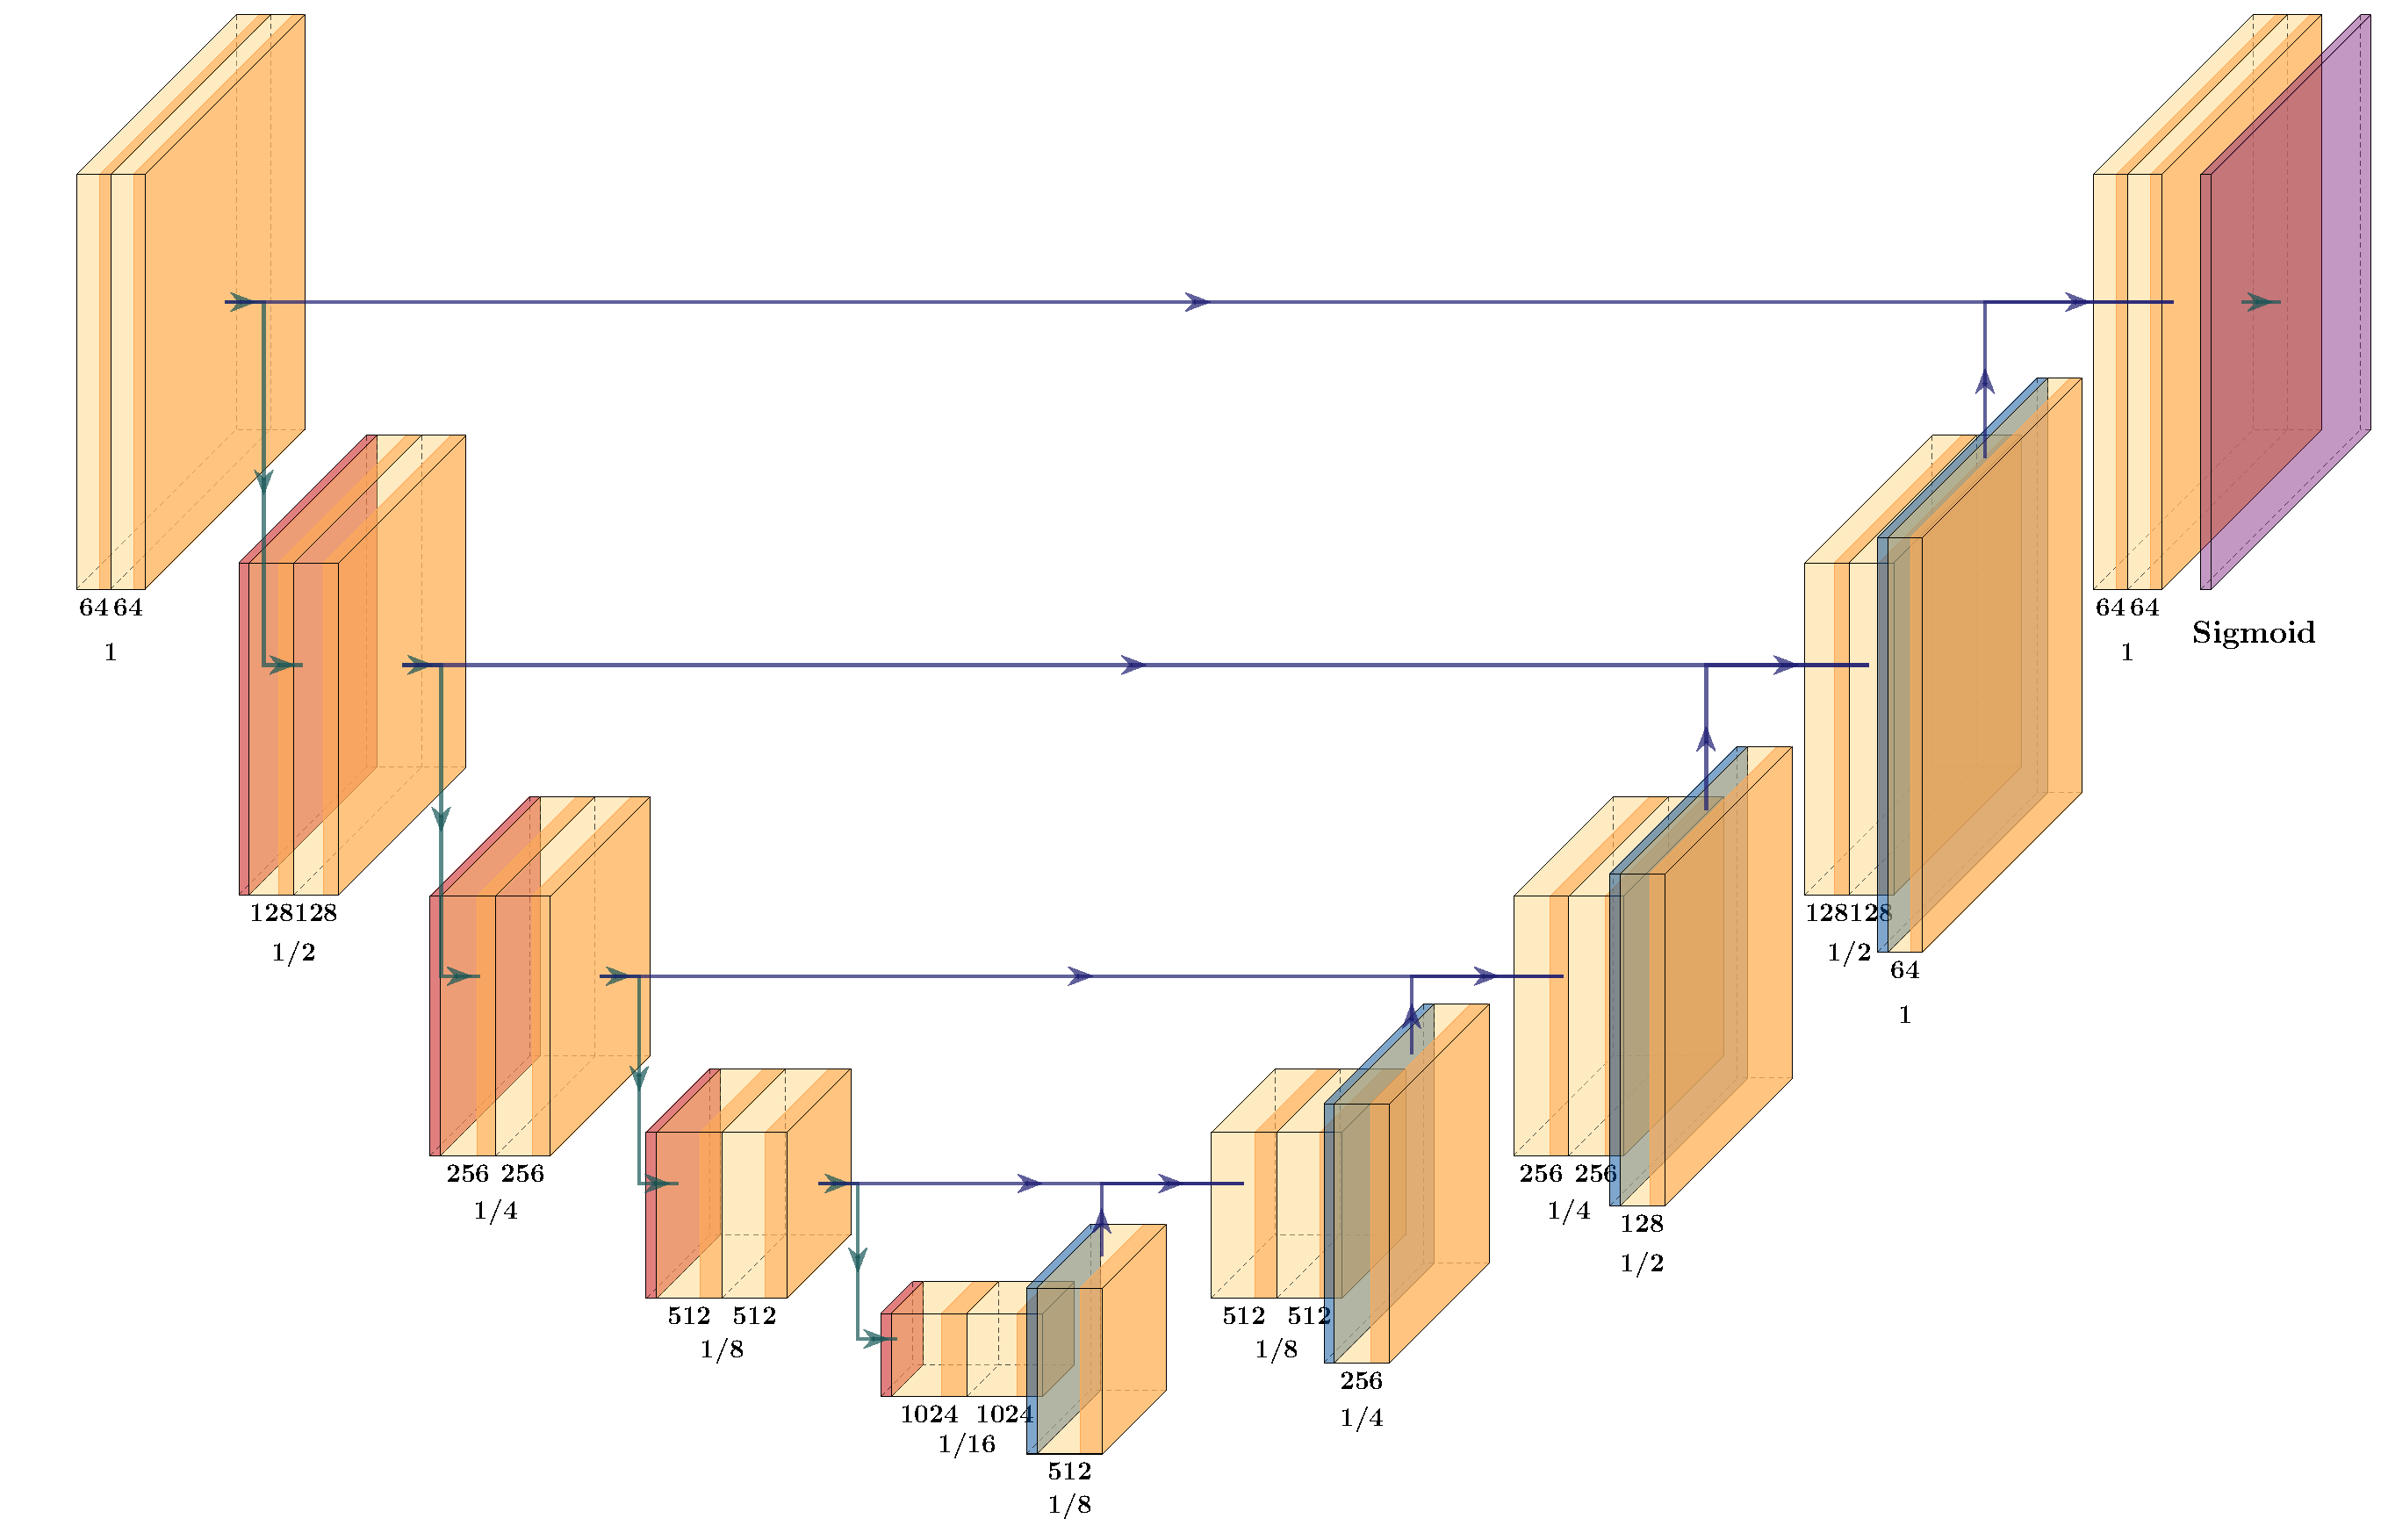
\includegraphics[width=1\textwidth]{images/U-Net.pdf}};
    
    \filldraw[color=\ConvColor, opacity=0.5] (0,1.5) rectangle (1,2.5);
    \draw[] (0,1.5) rectangle (1,2.5);
    \node[right] at (1, 2) {\scriptsize{3$\times$3 Convolution}};
    
    \filldraw[color=\ConvReluColor, opacity=0.8] (0,0) rectangle (1,1);
    \draw[] (0,0) rectangle (1,1);
    \node[right] at (1, 0.5) {\scriptsize{ReLU}};
    
    \filldraw[color=\PoolColor, opacity=0.75] (9,0) rectangle (10,1);
    \draw[] (9,0) rectangle (10,1);
    \node[right] at (10, 0.5) {\scriptsize{2$\times$2 Max-pooling}};
    
    \filldraw[color=\UnpoolColor, opacity=0.7] (9,1.5) rectangle (10,2.5);
    \draw[] (9,1.5) rectangle (10,2.5);
    \node[right] at (10, 2) {\scriptsize{2$\times$2 Up-convolution}};
    
    % \filldraw[color=\PoolColor, opacity=1] (18,0) rectangle (19,1);
    % \draw[] (18,0) rectangle (19,1);
    \node[right] at (19, 0.5) {\scriptsize{Feedforward}};
    
    % \filldraw[color=\PoolColor, opacity=1] (18,1.5) rectangle (19,2.5);
    % \draw[] (18,1.5) rectangle (19,2.5);
    \node[right] at (19, 2) {\scriptsize{Concatenation}};

    \begin{scope}[decoration={
        markings, mark=at position 0.75 with {\arrow[scale=1.5]{stealth}}}] 
        \draw[postaction={decorate}, color={rgb:blue,4;red,1;green,4;black,3}] (18,0.5)--(19,0.5);
        \draw[postaction={decorate}, color={rgb:blue,4;red,1;green,1;black,3}] (18,2)--(19,2);
    \end{scope}
\end{tikzpicture}
    \caption[A diagram of the U-Net architecture (created using an open-source CNN architecture visualisation tool). The architecture is named after the U-shape that it resembles when illustrated in this way. Each cube represents a layer with the number of output feature maps shown at the bottom of the cube. At the bottleneck there are 1024 feature maps that are each one sixteenth the size of the input image in the $x$ and $y$ dimensions. The green arrows represent the feedforward of information from one layer to the next, whereas the blue arrows represent the concatenation of the feature maps of one layer to another. Note that the max-pooling layers at the end of each contracting block are shown at the start of the next block for easier illustration of the pass forward of the feature channels. Similarly, the up-convolution layers are shown at the end of each contracting block rather than at the start of the next.]{A diagram of the U-Net architecture (created using an open-source CNN architecture visualisation tool\footnotemark). The architecture is named after the U-shape that it resembles when illustrated in this way. Each cube represents a layer with the number of output feature maps shown at the bottom of the cube. At the bottleneck there are 1024 feature maps that are each one sixteenth the size of the input image in the $x$ and $y$ dimensions. The green arrows represent the feedforward of information from one layer to the next, whereas the blue arrows represent the concatenation of the feature maps of one layer to another. Note that the max-pooling layers at the end of each contracting block are shown at the start of the next block for easier illustration of the pass forward of the feature channels. Similarly, the up-convolution layers are shown at the end of each contracting block rather than at the start of the next.}
    \label{fig:unetushape}
\end{figure}

\subsection{Training}

\footnotetext{\url{https://github.com/HarisIqbal88/PlotNeuralNet}}

Once the architecture and online data augmentation process had been implemented, the model was then compiled using the \texttt{compile} method from the \texttt{Model} class. The \texttt{compile} method can then be used to define which optimiser and loss function to use, and which metrics to monitor, and the \texttt{fit} method can be used to train the network.

\subsubsection{Keras Callbacks}

The Keras callbacks are objects that can perform actions at various stages of training (e.g., at the start or end of epochs or batches)\footnote{\url{https://keras.io/api/callbacks}}. Callbacks were used to implement early stopping, model checkpointing, and metric visualisation using TensorBoard\footnote{\url{https://www.tensorflow.org/tensorboard}}.

As discussed in Chapter \ref{chap:technical}, early stopping is a regularization technique in which the training process is stopped given some ``stopping criteria'' rather than after a set number of epochs. The Keras library allows users to implement early stopping using the \texttt{EarlyStopping} callback. Both the metric to monitor and a \texttt{patience} argument must be provided to the \texttt{EarlyStopping} callback. In this case, the loss achieved on the validation set is monitored. The \texttt{patience} argument defines the number of epochs that the validation loss can increase before the training is stopped.

Model checkpointing and TensorBoard visualisation are implemented with the \texttt{ModelCheckpoint} and \texttt{TensorBoard} callbacks respectively. The \texttt{ModelCheckpoint} callback simply saves the parameters of the entire network after each epoch to a \texttt{.hdf5} file. Using the \texttt{save\_best\_only=False} argument and a filename formatted using the current epoch number ensures that each epoch is saved as a new file, rather than the previous epoch's save being overwritten. Example usage of the callbacks discussed are shown in Listing \ref{lst:compile}.

\begin{figure}[t]
    \centering
    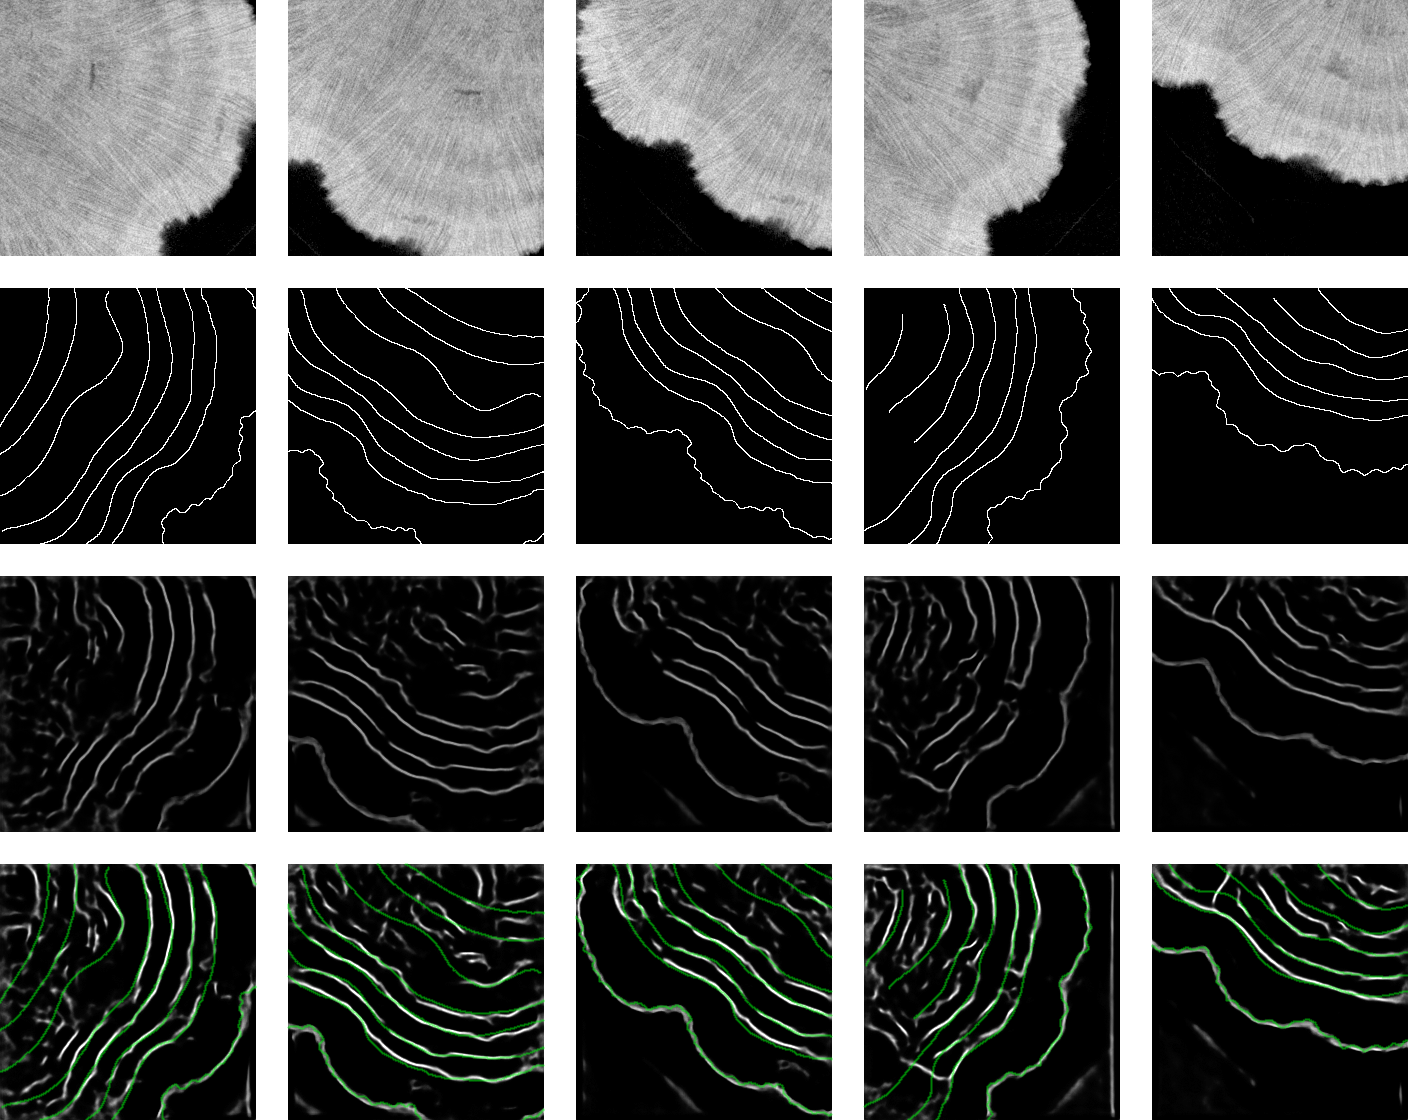
\includegraphics[width=1\textwidth]{images/initial-outputs.png}
    \caption{Initial results achieved by the network. Note that the hyperparameters chosen are not necessarily optimal and that performance may still be improved. \textbf{(top)} The input samples from the test set. \textbf{(center)} The ground truth labels. \textbf{(bottom)} The output labels.}
    \label{fig:outputs}
\end{figure}

\subsubsection{Initial Results}

A few examples of the initial results achieved are shown in Figure \ref{fig:outputs}. These initial results were output by a network trained using the Adam optimiser~\cite{adam} with a learning rate of 0.0001 to optimise the binary cross-entropy loss function. The network was trained for 20 epochs with each epoch consisting of 500 augmented samples. A batch size of two was used. An average per-pixel accuracy of 96.7\% was acheived. Note that this high accuracy is misleading and is discussed in Section \ref{sec:accimplementation}. The entire training process took ${\sim}$16 minutes on an Nvidia P100 ``Pascal'' GPU. Many more examples of boundary predictions resulting from networks trained with different hyperparameters are shown throughout Chapter \ref{chap:evaluation}. Listing \ref{lst:compile} shows a simplified example of the compilation of a network configured with these hyperparameters.

\section{Three Dimensional Boundary Extraction}
\label{sec:threedimension}

This section discusses the attempts to implement and train a modified U-Net architecture capable of extracting the annual density banding present in three dimensional data. As opposed to only utilising the density information a single slice, the modified architecture also makes use of the density information of surrounding slices when determining the boundary positions. An overview of the components implemented in this section is shown in Figure \ref{fig:3doverview}.

\begin{figure}[t]
    \centering
    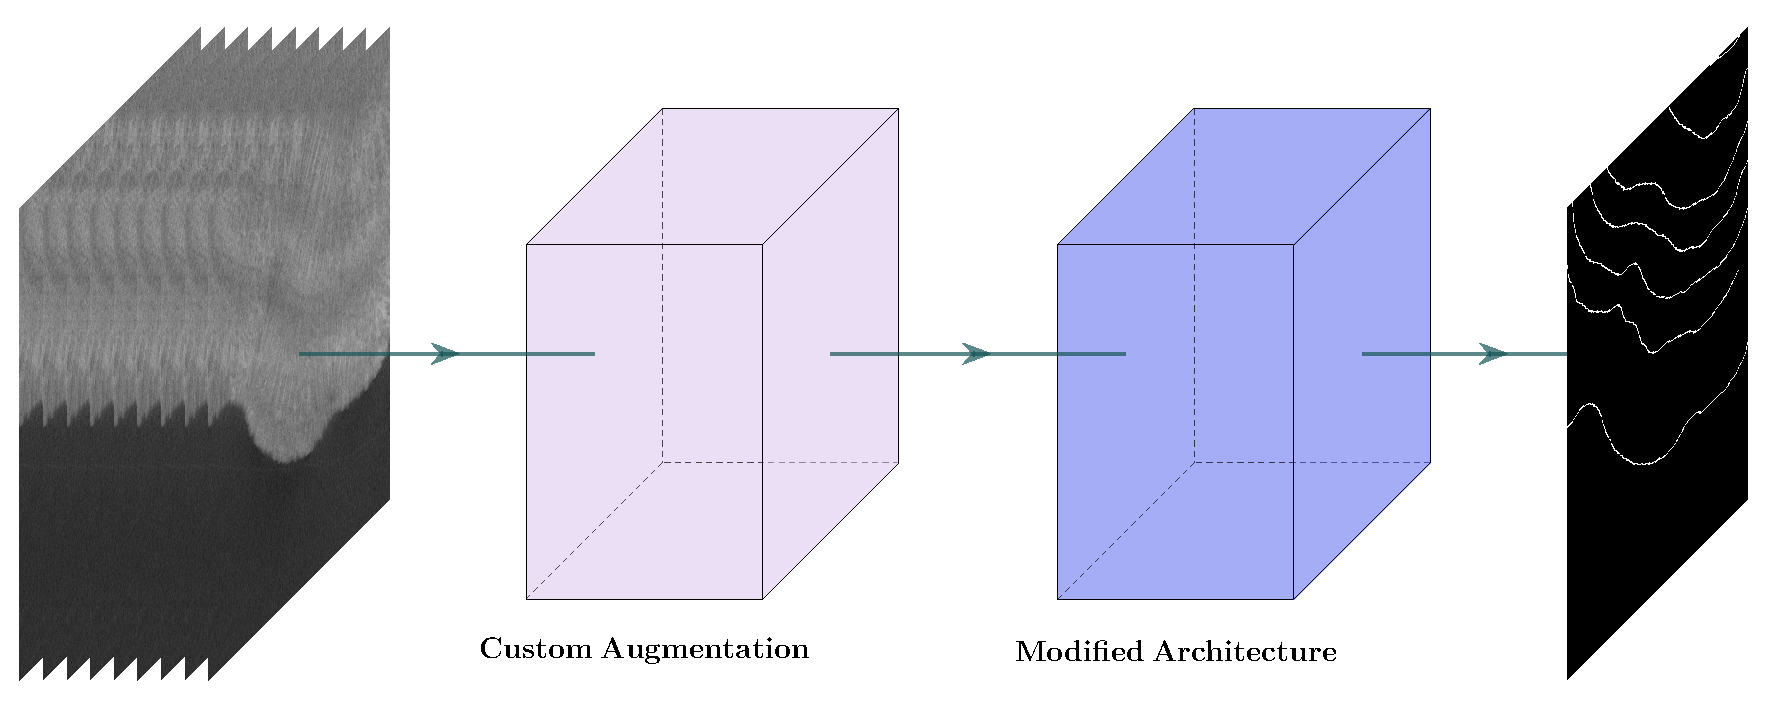
\includegraphics[width=0.95\textwidth]{images/3D-overview.pdf}
    \caption{An overview of the components implemented in this section. Each training sample that the modified architecture trains on will consist of nine patches. Only the centre slice is labelled and the model attempts to extract the boundaries present in this central slice. A custom 3D ``data loader'' is implemented in order to perform online augmentation of the nine-patch training samples.}
    \label{fig:3doverview}
\end{figure}

\subsection{Dataset Expansion}

In order to train the modified architecture, the curated dataset discussed in Section \ref{sec:datasetcuration} was expanded to include data from slices surrounding the slices initially labelled. Since the modified architecture makes use of up to nine slices (the central slice and four slices on either side), the eight slices surrounding the labelled slices also needed to be extracted. As mentioned in Section \ref{sec:2dlabel}, when the sliding window Python script was used to create the 2D dataset, patches from surrounding slices were also produced. The resulting 3D dataset contains the same amount of samples (388) with each sample consisting of nine patches and the label consisting of the central labelled patch. The nine-sample patches are stored with the same name as the label apart from a suffix of \texttt{\_0} to \texttt{\_8} denoting the patches' positions relative to the central patch which has a suffix of \texttt{\_4}.

\subsection{Data Loader Implementation}

Whereas the 2D architecture made use of the \texttt{ImageDataGenerator} class to load 2D images into the model, a 3D version of the \texttt{ImageDataGenerator} class is not currently implemented in the Keras library. Although the \texttt{ImageDataGenerator} class could be used to simply load nine patches one after another and the Keras \texttt{stack} method could be used to stack the images to produce a $(9 \times y \times x \times 1)$ tensor, this method would not allow for online augmentation to be performed since different random transformations would be applied to all nine of the loaded patches. Note also that even if the same transformations were able to be applied to each 2D patch, transformations in the third dimension would not be possible. Thus, a custom data loader was written.

An \texttt{ImageDataGenerator3D} class and a \texttt{LabelDataGenerator2D} class were implemented. These were designed to be similar to the Keras \texttt{ImageDataGenerator} class allowing the same data augmentation arguments to be passed to their constructors. Recall that in order to produce 2D image-label pairs, a pair of generators created using the \texttt{flow\_from\_directory} method were used with the same \texttt{seed} to augment the image-label pairs with the same transformations. The online augmentation of the 3D data is designed to follow a similar structure; a pair of generators created using the \texttt{flow\_from\_directory} method of the \texttt{ImageDataGenerator3D} and \texttt{LabelDataGenerator2D} classes with the same \texttt{seed} argument are used to perform online augmentation to both the nine-patch sample and the single label patch. The \texttt{ImageDataGenerator3D} class is used to load and augment the 3D samples and the \texttt{LabelDataGenerator2D} class is used to load and augment the 2D labels.

The \texttt{flow\_from\_directory} method of the \texttt{ImageDataGenerator3D} class first sorts the \texttt{.png} images from the sample directory alphanumerically. Nine images are then loaded, stacked, and ``unsqueezed'' resulting in a $(9 \times y \times x \times 1)$ tensor. The unsqueeze operation takes for example a $(y \times x)$ tensor and produces a $(y \times x \times 1)$ tensor. These stacks of nine images are then augmented using techniques discussed in Section \ref{sec:3daug} and are finally stacked into $(batch \times 9 \times y \times x \times 1)$ tensors where $batch$ is the batch size.

The \texttt{flow\_from\_directory} method of the \texttt{LabelDataGenerator2D} class also sorts the \texttt{.png} images from the label directory alphanumerically. These images are then loaded and unsqueezed resulting in a $(y \times x \times 1)$ tensors containing a single label. The appropriate augmentation transformations are then applied and the resulting tensors are stacked into $(batch \times y \times x \times 1)$ tensors.

The two generators produced by the \texttt{flow\_from\_directory} methods of the \texttt{ImageDataGenerator3D} and \texttt{LabelDataGenerator2D} classes were then zipped together to create a single generator that yielded sample-label pairs with the sample consisting of nine patches, and the label consisting of only the central label. Similarly to the Keras \texttt{flow\_from\_directory} methods used when loading and augmenting the 2D data, these custom methods could also accept a \texttt{seed} argument ensuring that the same transformations are applied to the sample-label pairs. The custom \texttt{flow\_from\_directory} method was also capable of shuffling the order in which samples and labels were loaded and \texttt{seed} argument ensured that the samples and labels were shuffled in the same order.

Example usage of the \texttt{ImageDataGenerator3D} and \texttt{LabelDataGenerator2D} classes in order to perform online 3D augmentation is shown in Listing \ref{lst:3Daugment}.

\subsection{Three Dimensional Data Augmentation}
\label{sec:3daug}

% The transformations implemented that made use of the third dimension were random rotations within a range 

% \begin{itemize}
%     \item Rotation rotations
% \end{itemize}

\subsection{Architecture Modification}

Although various modified architectures were experimented with and are discussed in Chapter \ref{chap:evaluation}, only the initial modified architecture experimented with will be described here.

At a high level, the modification consisted of replacing all of the 2D operations in the contracting path with their 3D counterparts. However, issues arise when a tensor output from a 3D layer is passed to a 2D layer. Whereas the Keras \texttt{Conv3D} layer requires an input tensor with shape ($batch \times z \times y \times x \times channels$) and produces a tensor with the same shape, the \texttt{Conv2D} layer inputs and outputs tensors with the shape ($batch \times y \times x \times channels$). Thus, in order to pass the resulting tensor to a 2D layer, the tensor of shape ($batch \times z \times y \times x \times channels$) must be reshaped into a ($batch \times y \times x \times (z \times channels)$) tensor.

% The implementation of the first block of the modified contracting path is shown in Listing 

% Although the nine-patch sample could simply be input into the 2D architecture as a 2D images with nine channels allowing the network to make use of nine patches as opposed to one, an input tensor of this shape would not enable 3D convolutions. Without the use of 3D convolutions, the network can not make 

% The modified architecture does not perform as well as the 2D architecture. Inspecting the results both ... are shown in Chapter \ref{chap:evaluation}.

\subsection{Fully Three Dimensional Architecture}

% there was a fully 3d architecture where all 2d were replaced with 3d but not good performance at all. required 9 labelled slices as opposed to 1 central one and so very few sample-label pairs could be created. Discussed in Chapter \ref{chap:evaluation}.

% \newpage

\section{Accuracy Metric Implementation}
\label{sec:accimplementation}

As discussed briefly in Chapter \ref{chap:context}, choosing an appropriate accuracy metric for the boundary extraction task was particularly challenging. This section discusses the need for a custom accuracy metric and then details its implementation.

\subsection{Motivation}

There are two major issues that arise when using a standard per-pixel accuracy metric to quantify the performance achieved in this task. The first issue stems from the severe class imbalance present in the labels. On average, ${\sim}$98\% of a labelled patch is black---part of the ``not part of a boundary'' class. As a result, a model that learned to output a pure black image would achieve an average accuracy of 98\%. The inherent class imbalance gives rise to another problem when assessing the performance of the model. Since the boundary labels are only one pixel wide, a model predicting boundary positions just one pixel to the left or right could achieve an accuracy of 0\%. A custom accuracy metric must be conceived in order to reward a model even in predicting a boundary a few pixels away from the manually labelled position. Eventually, a metric based off of the average euclidean distances between the predicted and ground truth boundaries was designed.

\subsection{Overview}

\subsection{Skeletonisation}

\begin{figure}[t]
    \centering
    \begin{subfigure}[t]{0.32\textwidth}
        \centering
        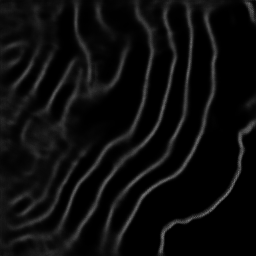
\includegraphics[width=1\textwidth, valign=c]{images/skel-pred.png}
    \end{subfigure}
    ~
    \begin{subfigure}[t]{0.32\textwidth}
        \centering
        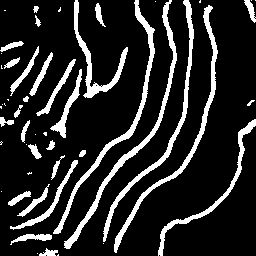
\includegraphics[width=1\textwidth, valign=c]{images/skel-thresh.png}
    \end{subfigure}
    ~
    \begin{subfigure}[t]{0.32\textwidth}
        \centering
        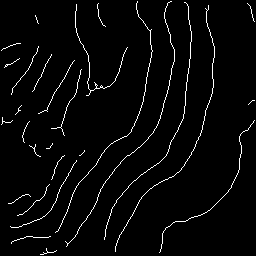
\includegraphics[width=1\textwidth, valign=c]{images/skel-skel.png}
    \end{subfigure}
    \caption{Skeletonisation example.....}
    \label{fig:skeletonisation}
\end{figure}

\begin{algorithm}[t]
    
    \For{$i=0$ {\bf upto} $n$}{
      $t_i \leftarrow 0$\;
    }
    \caption{This is an example algorithm.}
    \label{alg:accuracy}
\end{algorithm}

(Show algorithm and maybe some source code?) In Algorithm \ref{alg:accuracy}.

\subsection{Average Distance Calculation}

\subsection{The \texttt{ctypes} Module}

% \newpage

\section{Calcification Rate Estimation}

\subsection{Point Sampling}